\documentclass[border=10pt]{standalone}
\usepackage{tikz}
\usetikzlibrary{arrows.meta, calc, angles, quotes, decorations.markings}

\begin{document}
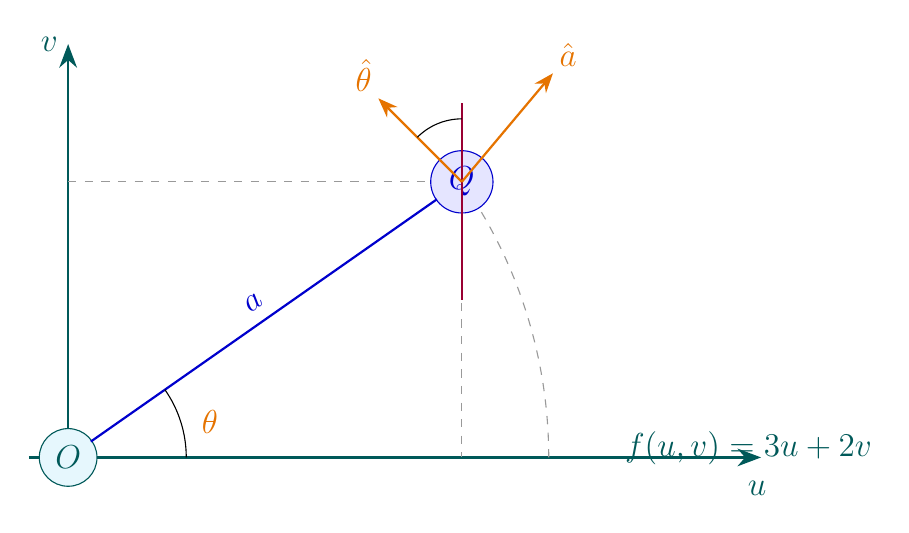
\begin{tikzpicture}[
    >=Stealth, % Set default arrow tip style
    font=\large,
    ]
    % Define colors to match the image
    \colorlet{myblue}{blue!80!black}
    \colorlet{myorange}{orange!90!black}
    \colorlet{myteal}{teal!70!black}
    \colorlet{mypurple}{purple!80!black}
    \colorlet{pointfill}{blue!10}
    \colorlet{dashcolor}{gray!80}

    % Define key coordinates
    \coordinate (O) at (0,0);
    \coordinate (Q) at (5,3.5);
    
    % Calculate angle and radius for Q
    \pgfmathsetmacro{\angleQ}{atan(3.5/5)}
    \pgfmathsetmacro{\radiusQ}{sqrt(5^2+3.5^2)}

    % Draw the u and v axes
    \draw[myteal, thick, -{Stealth[length=3mm]}] (-0.5,0) -- (8.8,0);
    \draw[myteal, thick, -{Stealth[length=3mm]}] (0,-0.35) -- (0,5.25) node[left] {$v$};

    % Place the function expression and the 'u' label on the horizontal axis
    \node[anchor=west, text=myteal] at (6.95,0.12) {$f(u,v)=3u+2v$};
    \node[text=myteal, anchor=north] at (8.75,-0.18) {$u$};

    % Draw dashed helper lines and arc
    \draw[dashed, dashcolor] (O |- Q) -- (Q) -- (O -| Q);
    \draw[dashed, dashcolor] (\radiusQ, 0) arc (0:\angleQ:\radiusQ);

    % Draw the origin point 'O'
    \node[circle, draw=myteal, fill=cyan!10, inner sep=3pt, text=myteal] at (O) {$O$};
    
    % Draw the point 'Q'
    \node[circle, draw=myblue, fill=pointfill, inner sep=3pt, text=myblue] at (Q) {$Q$};

    % Draw the position vector 'a' from O to Q
    \draw[myblue, thick, shorten <=10pt, shorten >=11pt] (O) -- (Q) node[midway, sloped, above, yshift=1pt, text=myblue] {$a$};

    % Draw the angle theta at the origin
    \coordinate (X_axis_point) at (1.5,0);
    \pic[draw, decoration={markings, mark=at position 0.5 with {\arrow{<}}}, postaction={decorate}, angle radius=1.5cm] {angle=X_axis_point--O--Q};
    \node[myorange] at (1.8, 0.45) {$\theta$};

    % Draw the vertical line through Q
    \draw[mypurple, thick] (Q |- 0,2) -- (Q |- 0,4.5);

    % Draw the unit vectors at Q
    \draw[myorange, thick, -{Stealth[length=2.5mm]}] (Q) -- ++(50:1.8) node[anchor=south west, inner sep=2pt, text=myorange] {$\hat{a}$};
    \draw[myorange, thick, -{Stealth[length=2.5mm]}] (Q) -- ++(135:1.5) node[anchor=south east, inner sep=2pt, text=myorange] {$\hat{\theta}$};

    % Draw the angle at Q
    \coordinate (V_line_point) at ($(Q)+(0,0.8)$);
    \coordinate (Theta_hat_point) at ($(Q)+(135:0.8)$);
    \pic[draw, angle radius=0.8cm] {angle=V_line_point--Q--Theta_hat_point};

\end{tikzpicture}
\end{document}
